% Template of basic phisics experiment 基于 article template,在此基础上做修改
% 设定文章编码类型,正文字号为五号则 zihao=5,正文字号为小四则 zihao=-4
\documentclass[zihao=5, UTF8]{article}		


% 自定义宏定义
\def\N{\mathbb{N}}
\def\F{\mathbb{F}}
\def\Z{\mathbb{Z}}
\def\Q{\mathbb{Q}}
\def\R{\mathbb{R}}
\def\C{\mathbb{C}}
\def\T{\mathbb{T}}
\def\S{\mathbb{S}}
\def\A{\mathbb{A}}
\def\I{\mathscr{I}}
\def\d{\mathrm{d}}
\def\p{\partial}


% 物理实验报告所需的其它宏包
\usepackage{ulem}   % \uline 下划线支持

% 导入基本宏包
\usepackage[UTF8]{ctex}     % 设置文档为中文语言
\usepackage[colorlinks, linkcolor=blue, anchorcolor=blue, citecolor=blue, urlcolor=blue]{hyperref}  % 宏包:自动生成超链接 (此宏包与标题中的数学环境冲突)
% \usepackage{docmute}    % 宏包:子文件导入时自动去除导言区,用于主/子文件的写作方式,\include{./51单片机笔记}即可。注:启用此宏包会导致.tex文件capacity受限。
\usepackage{amsmath}    % 宏包:数学公式
\usepackage{mathrsfs}   % 宏包:提供更多数学符号
\usepackage{amssymb}    % 宏包:提供更多数学符号
\usepackage{pifont}     % 宏包:提供了特殊符号和字体
\usepackage{extarrows}  % 宏包:更多箭头符号

% 列表环境设置
\usepackage{enumitem}   % 宏包:列表环境设置
    \setlist[enumerate]{itemsep=0pt, parsep=0pt, topsep=0pt, partopsep=0pt, leftmargin=3.5em} 
    \setlist[itemize]{itemsep=0pt, parsep=0pt, topsep=0pt, partopsep=0pt, leftmargin=3.5em}
    \newlist{circledenum}{enumerate}{1} % 创建一个新的枚举环境  
    \setlist[circledenum,1]{  
        label=\protect\circled{\arabic*}, % 使用 \arabic* 来获取当前枚举计数器的值,并用 \circled 包装它  
        ref=\arabic*, % 如果需要引用列表项,这将决定引用格式(这里仍然使用数字)
        itemsep=0pt, parsep=0pt, topsep=0pt, partopsep=0pt, leftmargin=3.5em
    }  
% 文章页面 margin 设置
\usepackage[a4paper]{geometry}  % 宏包:文章页面 margin 设置
    \geometry{top=0.75in}
    \geometry{bottom=0.75in}
    \geometry{left=0.75in}
    \geometry{right=0.75in}   % 设置上下左右页边距
    \geometry{marginparwidth=1.75cm}    % 设置边注距离(注释、标记等)

% 自定义数学环境
\usepackage{amsthm} % 宏包:数学环境配置
% theorem-line 环境自定义
    \newtheoremstyle{MyLineTheoremStyle}% <name>
        {11pt}% <space above>
        {11pt}% <space below>
        {}% <body font> 使用默认正文字体
        {}% <indent amount>
        {\bfseries}% <theorem head font> 设置标题项为加粗
        {:}% <punctuation after theorem head>
        {.5em}% <space after theorem head>
        {\textbf{#1}\thmnumber{#2}\ \ (\,\textbf{#3}\,)}% 设置标题内容顺序
    \theoremstyle{MyLineTheoremStyle} % 应用自定义的定理样式
    \newtheorem{LineTheorem}{Theorem.\,}
% theorem-block 环境自定义
    \newtheoremstyle{MyBlockTheoremStyle}% <name>
        {11pt}% <space above>
        {11pt}% <space below>
        {}% <body font> 使用默认正文字体
        {}% <indent amount>
        {\bfseries}% <theorem head font> 设置标题项为加粗
        {:\\ \indent}% <punctuation after theorem head>
        {.5em}% <space after theorem head>
        {\textbf{#1}\thmnumber{#2}\ \ (\,\textbf{#3}\,)}% 设置标题内容顺序
    \theoremstyle{MyBlockTheoremStyle} % 应用自定义的定理样式
    \newtheorem{BlockTheorem}[LineTheorem]{Theorem.\,} % 使用 LineTheorem 的计数器
% definition 环境自定义
    \newtheoremstyle{MySubsubsectionStyle}% <name>
        {11pt}% <space above>
        {11pt}% <space below>
        {}% <body font> 使用默认正文字体
        {}% <indent amount>
        {\bfseries}% <theorem head font> 设置标题项为加粗
        {:\\ \indent}% <punctuation after theorem head>
        {0pt}% <space after theorem head>
        {\textbf{#3}}% 设置标题内容顺序
    \theoremstyle{MySubsubsectionStyle} % 应用自定义的定理样式
    \newtheorem{definition}{}


% 有色文本框及其设置
\usepackage[dvipsnames,svgnames]{xcolor}    %设置插入的文本框颜色
\usepackage[strict]{changepage}     % 提供一个 adjustwidth 环境
\usepackage{framed}     % 实现方框效果
    \definecolor{graybox_color}{rgb}{0.95,0.95,0.96} % 文本框颜色。修改此行中的 rgb 数值即可改变方框纹颜色,具体颜色的rgb数值可以在网站https://colordrop.io/ 中获得。(截止目前的尝试还没有成功过,感觉单位不一样)(找到喜欢的颜色,点击下方的小眼睛,找到rgb值,复制修改即可)
    \newenvironment{graybox}{%
    \def\FrameCommand{%
    \hspace{1pt}%
    {\color{gray}\small \vrule width 2pt}%
    {\color{graybox_color}\vrule width 4pt}%
    \colorbox{graybox_color}%
    }%
    \MakeFramed{\advance\hsize-\width\FrameRestore}%
    \noindent\hspace{-4.55pt}% disable indenting first paragraph
    \begin{adjustwidth}{}{7pt}%
    \vspace{2pt}\vspace{2pt}%
    }
    {%
    \vspace{2pt}\end{adjustwidth}\endMakeFramed%
    }

% 各级标题自定义设置
\usepackage{titlesec}   
    % section标题自定义设置 
    \titleformat{\section}[hang]{\normalfont\huge\bfseries\centering}{第\,\thesection\,部分}{20pt}{}
    % subsection标题自定义设置 
    \titleformat{\subsection}[hang]{\normalfont\Large\bfseries}{\,\thesubsection\,}{8pt}{}
    % subsubsection标题自定义设置
    \titleformat{\subsubsection}[hang]{\normalfont\large\bfseries}{\,\thesubsubsection\,}{6pt}{}

% 外源代码插入设置
\usepackage{matlab-prettifier}
    \lstset{
        style=Matlab-editor,  % 继承matlab代码颜色等
    }
\usepackage[most]{tcolorbox} % 引入tcolorbox包 
\usepackage{listings} % 引入listings包
    \tcbuselibrary{listings, skins, breakable}
    \lstdefinestyle{matlabstyle}{
        language=Matlab,
        basicstyle=\small,
        breakatwhitespace=false,
        breaklines=true,
        captionpos=b,
        keepspaces=true,
        numbers=left,
        numbersep=15pt,
        showspaces=false,
        showstringspaces=false,
        showtabs=false,
        tabsize=2
    }
    \newtcblisting{matlablisting}{
        arc=0pt,
        top=0pt,
        bottom=0pt,
        left=1mm,
        listing only,
        listing style=matlabstyle,
        breakable,
        colback=white   % 选一个合适的颜色
    }

% table 支持
\usepackage{booktabs}   % 宏包:三线表
\usepackage{tabularray} % 宏包:表格排版
\usepackage{longtable}  % 宏包:长表格
\usepackage{tabularx}  % 宏包:宽表格
\usepackage{multirow}  % 宏包:表格中一格显示多个项目

% figure 设置
\usepackage{graphicx}  % 支持 jpg, png, eps, pdf 图片 
\usepackage{svg}       % 支持 svg 图片
    \svgsetup{
        % 指向 inkscape.exe 的路径
        inkscapeexe = C:/aa_MySame/inkscape/bin/inkscape.exe, 
        % 一定程度上修复导入后图片文字溢出几何图形的问题
        inkscapelatex = false                 
    }


% 图表进阶设置
\usepackage{float}     % 图表位置浮动设置 
\usepackage{caption}    % 图注、表注
    \captionsetup[figure]{name=图}  
    \captionsetup[table]{name=表}
    \captionsetup{labelfont=bf, font=small}

% 文章默认字体设置
    \usepackage{fontspec}   % 宏包:字体设置
       \setmainfont{SimSun}    % 设置中文字体为宋体字体
      \setCJKmainfont[AutoFakeBold=3]{SimSun} % 设置加粗字体为 SimSun 族,AutoFakeBold 可以调整字体粗细^     \setmainfont{Times New Roman} % 设置英文字体为Times New Roman


% 其它设置
    % equation 公式编号设置
        \makeatletter  
        \renewcommand{\theequation}{\thesection.\arabic{equation}}  
        \makeatother
    % 脚注设置
        \renewcommand\thefootnote{\ding{\numexpr171+\value{footnote}}}
    % 参考文献引用设置
        \bibliographystyle{unsrt}   % 设置参考文献引用格式为unsrt
        \newcommand{\upcite}[1]{\textsuperscript{\cite{#1}}}     % 自定义上角标式引用
    % 文章序言设置
        \newcommand{\cnabstractname}{序言}
        \newenvironment{cnabstract}{%
            \par\Large
            \noindent\mbox{}\hfill{\bfseries \cnabstractname}\hfill\mbox{}\par
            \vskip 2.5ex
            }{\par\vskip 2.5ex}


% 页眉页脚设置
\usepackage{fancyhdr}   %宏包:页眉页脚设置
    \pagestyle{fancy}
    \fancyhf{}
    \cfoot{\thepage}
    \renewcommand\headrulewidth{1pt}
    \renewcommand\footrulewidth{0pt}
    %\rhead{\bfseries 分组序号: YK04-2}    
    \chead{《数字电路》实验报告,\ 韩初晓,\ 2023K8009908002}
    \lhead{2024.10.17}

% 文档信息设置
%\title{这里是标题\\The Title of the Report}
%\author{丁毅\\ \footnotesize 中国科学院大学,北京 100049\\ Yi Ding \\ %\footnotesize University of Chinese Academy of Sciences, Beijing %100049, China}
%\date{\footnotesize 2024.8 -- 2025.1}

% 开始编辑文章

\begin{document}
%\noindent\begin{flushright}
%   \zihao{2}{分组序号: YK04-2}
%\end{flushright}

\setCJKfamilyfont{boldsong}[AutoFakeBold = {2.17}]{SimSun}
\newcommand*{\boldsong}{\CJKfamily{boldsong}}


\begin{center}\large
    \noindent{\Huge\bfseries\boldsong《数字电路》实验报告 }
    \\\vspace{0.4cm}
    \noindent\textit{
        \textbf{\boldsong 实验名称:}\uline{\hspace{1.7cm} 熟悉 vivado 环境\hspace{1.7cm}}\hspace{0.4cm} 
        指导教师:\uline{\hspace{1.0cm}王珎,范志华\hspace{1.0cm}}}
    \\\vspace{0.1cm}
    \noindent\textit{
        姓名:\uline{\,\,\,韩初晓\,\,\,}\hspace{0.2cm}
        学号:\uline{\,\,\,{\upshape 2023K8009908002}\,\,\,}\hspace{0.2cm}
        专业:\uline{\,\,\,计算机科学与技术\,\,\,}\hspace{0.2cm}
        班级:\uline{\,\,\,\upshape{2306}\,\,\,}}
    \\\vspace{0.1cm}
    \noindent\textit{
        实验日期:\uline{\,\,{\upshape 2024.10.17}\,\,}\hspace{0.2cm}
        实验地点:\uline{\,\,\,教学楼{\upshape221}\,\,\,}\hspace{0.2cm}
        是否调课/补课:\uline{\hspace{0.5cm}否\hspace{0.5cm}}\hspace{0.2cm}
        成绩:\uline{\hspace{2cm}}}
\end{center}
% \vspace{-0.2cm}
\noindent\rule{\textwidth}{0.1em}   % 分割线

% 控制目录不换页
\vspace{1cm}
\setcounter{tocdepth}{2}  % 目录深度为 2(不显示 subsubsection)
\noindent\begin{minipage}{\textwidth}\centering
\tableofcontents\thispagestyle{fancy}   % 显示页码、页眉等   
\end{minipage}  
\newpage

\section{实验目的}\thispagestyle{fancy} 
\begin{enumerate}
    \item 熟悉 Vivado 设计流程(设计$\rightarrow$仿真$\rightarrow$综合$\rightarrow$优化$\rightarrow$门级仿真$\rightarrow$电路制造工艺文件)
    \item 掌握Verilog的基本程序结构,掌握利用 Vivado 创建设计的方法(以实现 4 位加法器为例)
    \item 掌握编写 Testbench 的方法,以及行为仿真方法
\end{enumerate}

\subsection{实验环境}
\begin{itemize}
    \item Vivado 2017.4 开发工具
    \item FPGA 开发平台(根据手册中的默认设置进行选择)
\end{itemize}


\section{实验内容}
\subsection{实验一:实现四位加法器}
\subsubsection{原理说明}
四位加法器接受两个四位的二进制输入和一个进位输入,输出四位的和和一个进位输出。
我的代码中,加法器可以表示为:
\[
\{cout, out\} = in\_0 + in\_1 + cin
\]
其中,\texttt{cout} 是加法运算中的进位输出,\texttt{out} 是四位加法的结果。
\subsubsection{接口定义}
\begin{itemize}
    \item 输入信号:
    \begin{itemize}
        \item \texttt{in\_0[3:0]}:四位二进制数的第一个加数。
        \item \texttt{in\_1[3:0]}:四位二进制数的第二个加数。
        \item \texttt{cin}:输入进位信号,用于处理来自前一级的进位。
    \end{itemize}
    \item 输出信号:
    \begin{itemize}
        \item \texttt{out[3:0]}:四位加法运算的结果。
        \item \texttt{cout}:加法运算的进位输出信号,表示最高位的进位。
    \end{itemize}
\end{itemize}
\subsubsection{调试过程及结果}
 `add\_4' 模块,用于实现四位加法器,通过编写 Testbench 模块 `test\_add\_4' 对 `add\_4' 进行仿真测试,仿真波形展示了输入信号的变化以及对应的输出结果如下:
 \begin{figure}[htbp]
    \centering
    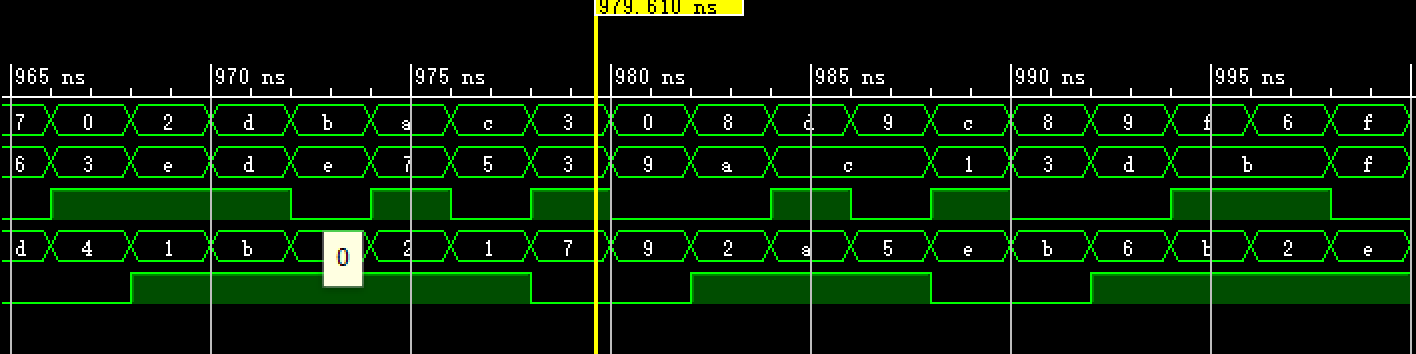
\includegraphics[width=\textwidth]{add_4.png} % 图片路径和大小
    \caption{add\_4模块的测试结果}
    \label{fig:add_4模块的测试结果}
\end{figure}


\subsection{实验二:实现一位加法器}

\subsubsection{原理说明}
一位加法器接受两个单比特二进制输入和一个进位输入,产生一个二进制和和一个进位输出。它可以用如下的逻辑表达式写出:
\[
\text{sum} = in\_a \oplus in\_b \oplus cin
\]
\[
\text{cout} = (in\_a \land in\_b) \lor ((in\_a \oplus in\_b) \land cin)
\]
其中:
 \( in\_a \) 和 \( in\_b \) 是两个单比特输入。
 \( cin \) 是进位输入。
 \( sum \) 是和输出。
 \( cout \) 是进位输出。
\subsubsection{接口定义}
\begin{itemize}
    \item 输入信号:
    \begin{itemize}
        \item \texttt{in\_a}:第一个加数。
        \item \texttt{in\_b}:第二个加数。
        \item \texttt{cin}:进位输入。
    \end{itemize}
    \item 输出信号:
    \begin{itemize}
        \item \texttt{sum}:加法运算的和。
        \item \texttt{cout}:进位输出。
    \end{itemize}
\end{itemize}
\subsubsection{调试过程及结果}
`add\_1' 模块实现了一位加法器,Testbench 模块 `test\_add\_1' 对 `add\_1' 进行仿真测试,结果波形图如下:
\begin{figure}[htbp]
    \centering
    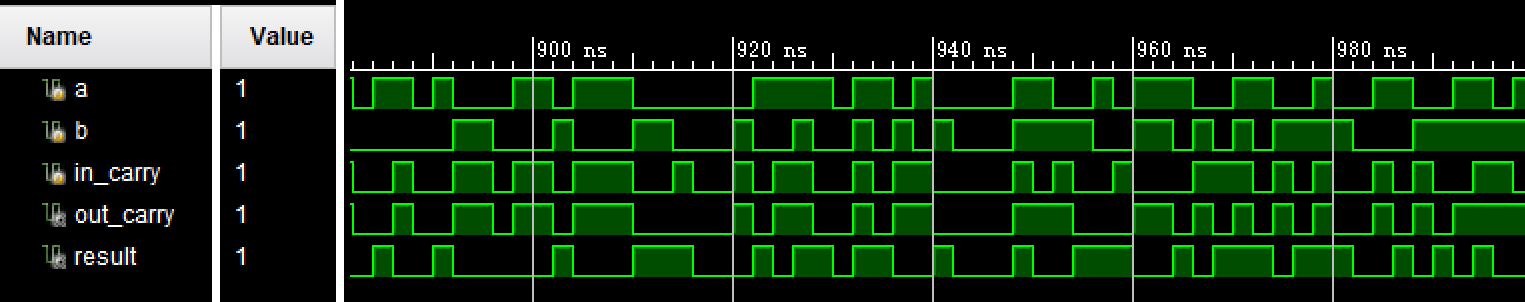
\includegraphics[width=\textwidth]{add_1.png} % 图片路径和大小
    \caption{add\_1模块的测试结果}
    \label{fig:add_1模块的测试结果}
\end{figure}


\subsection{实验三:实现三八译码器}
\subsubsection{原理说明}
三八译码器将输入的三位二进制数(0-7)转换为八个输出线其中一个的高电平,其他输入线保持低电平。每个输入值只激活一个输出信号。同时,在本实验中实现的三八译码器具有只有控制信号在高电平的情况下译码器才工作的动能。

三八译码器的真值表如下:
\begin{table}[H]
    \centering
    \caption{三八译码器真值表}
    \begin{tabular}{|c|c|c|c|c|c|c|c|c|}
        \hline
        输入 & 输出 \\
        \hline
        000 & 00000001 \\
        001 & 00000010 \\
        010 & 00000100 \\
        011 & 00001000 \\
        100 & 00010000 \\
        101 & 00100000 \\
        110 & 01000000 \\
        111 & 10000000 \\
        \hline
    \end{tabular}
\end{table}
\subsubsection{接口定义}
\begin{itemize}
    \item 输入信号:
    \begin{itemize}
        \item \texttt{in[2:0]}:三位二进制输入信号。
    \end{itemize}
    \item 输出信号:
    \begin{itemize}
        \item \texttt{out[7:0]}:八位输出信号,输出时只有一个为 1,其余都为 0。
    \end{itemize}
        \item 控制信号:
    \begin{itemize}
        \item \texttt{signal}:一位控制信号,控制信号为高电平时,译码器工作。
    \end{itemize}
\end{itemize}
\subsubsection{调试过程及结果}
`decoder' 模块实现了三八译码器, Testbench 模块 `test\_decoder' 对 `decoder' 进行仿真,仿真结果如下:
\begin{figure}[htbp]
    \centering
    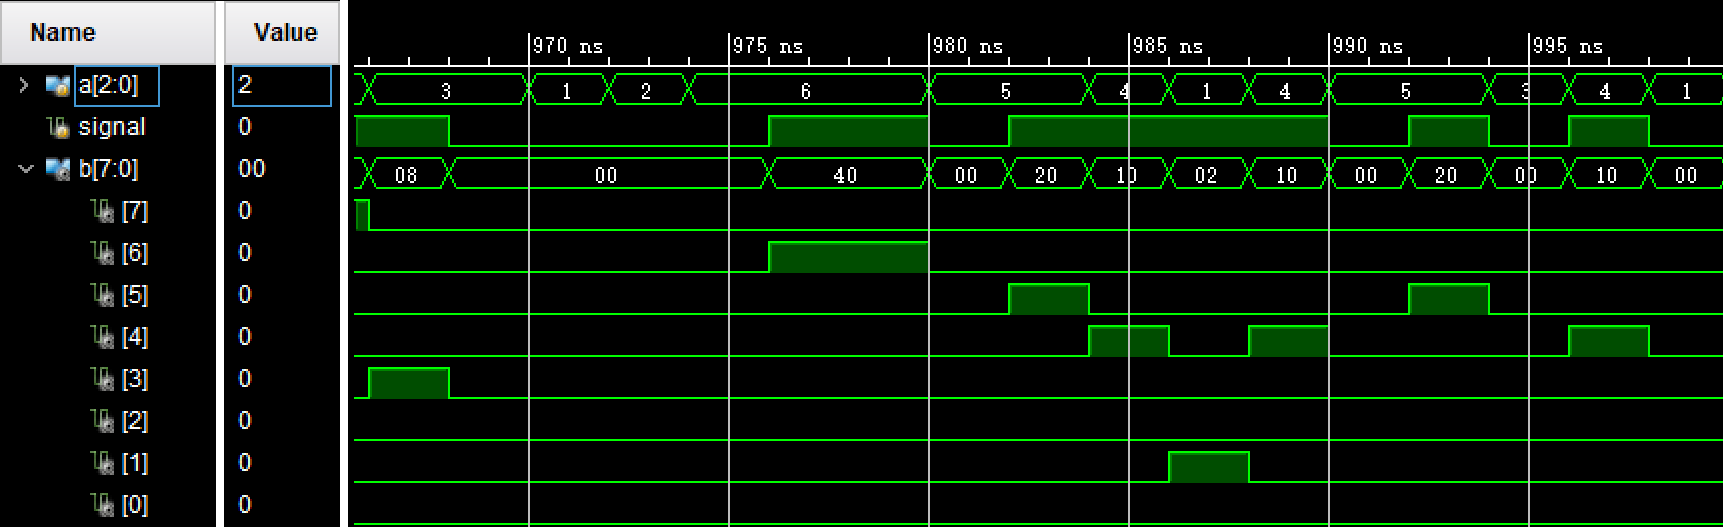
\includegraphics[width=\textwidth]{decoder.png} % 图片路径和大小
    \caption{decoder模块的测试结果}
    \label{fig:decoder模块的测试结果}
\end{figure}


\section{实验总结}
在本实验中我通过 Verilog 实现了数字电路中三个重要的模块——四位加法器、一位加法器和三八译码器。在亲手进行代码编写的时候,我更深入的理解了“行为级”和“结构级”的等价性,同时,我也更清楚的感受到了一些容易犯错的代码规范问题,提高了我使用Verilog语言进行硬件描述的能力。同时,我也学会了编写测试模块,这对于仿真验证的过程是十分重要的。

\section{源代码}
\subsection{实验一:实现四位加法器}
\begin{verbatim}
// this is the add_4 module
module add_4(
    input [3:0] in_0,
    input [3:0] in_1,
    input cin,
    output cout,
    output [3:0] out
    );
    assign {cout, out} = in_0 + in_1 + cin;
endmodule

// this is the test_add_4 module
module test_add_4()(
    .in_0(a),
    .in_1(b),
    .cin(in_carry),
    .out(sum),
    .cout(out_carry)
  );

  initial begin
    a = 4'h1;
    b = 4'h0;
    in_carry = 1'b0;
  end

  always begin
    #2;
    a = $random() % 16;
    b = $random() % 16;
    in_carry = $random() % 2;
  end
endmodule

\end{verbatim}

\subsection{实验二:实现一位加法器}
\begin{verbatim}
// this is the add_1 module
module add_1(
    input in_a,
    input in_b,
    input cin,
    output cout,
    output sum
    );
    assign sum = in_a ^ in_b ^ cin;
    assign cout = (in_a & in_b) | ((in_a ^ in_b) & cin);
endmodule

// this is the test_add_1 module
module test_add_1();
    reg a;
    reg b;
    reg in_carry;
    wire out_carry;
    wire result;

    add_1 instance_add1(
      .in_a(a),
      .in_b(b),
      .cin(in_carry),
      .cout(out_carry),
      .sum(result)
    );
    initial begin
      a = 1'b1;
      b = 1'b0;
      in_carry = 1'b0;
    end
    always begin
      #2;
      a = $random() % 2;
      b = $random() % 2;
      in_carry = $random() % 2;
    end
endmodule
\end{verbatim}

\subsection{实验三:实现三八译码器}
\begin{verbatim}
//this is the decoder module
module decoder(
    input [2:0] in,
    input signal,
    output reg [7:0] out
    );
    always @(*) begin
      out = 8'b00000000;
      if (signal) begin
      case (in)
        3'b001: out[1] = 1; 
        3'b010: out[2] = 1; 
        3'b011: out[3] = 1; 
        3'b100: out[4] = 1; 
        3'b101: out[5] = 1; 
        3'b110: out[6] = 1; 
        3'b111: out[7] = 1; 
        3'b000: out[0] = 1;  
      endcase
    end
    end
endmodule

//this is the test_decoder module
module test_decoder();
    reg [2:0] a;
    reg signal;
    wire [7:0] b;
    decoder instance_decoder(
      .in(a), .out(b), .signal(signal)
    );
initial begin
  a = 3'b000;
end
always begin
  #2;
  signal = $random() % 2;
  a = $random() % 8;
end
endmodule
\end{verbatim}

\end{document}

% VScode 常用快捷键:

% F2:                       变量重命名
% Ctrl + Enter:             行中换行
% Alt + up/down:            上下移行
% 鼠标中键 + 移动:           快速多光标
% Shift + Alt + up/down:    上下复制
% Ctrl + left/right:        左右跳单词
% Ctrl + Backspace/Delete:  左右删单词    
% Shift + Delete:           删除此行
% Ctrl + J:                 打开 VScode 下栏(输出栏)
% Ctrl + B:                 打开 VScode 左栏(目录栏)
% Ctrl + `:                 打开 VScode 终端栏
% Ctrl + 0:                 定位文件
% Ctrl + Tab:               切换已打开的文件(切标签)
% Ctrl + Shift + P:         打开全局命令(设置)

% Latex 常用快捷键:

% Ctrl + Alt + J:           由代码定位到PDF


